\documentclass[tikz]{standalone}
\usepackage{pgfplots}
\pgfplotsset{compat=1.15}
\usepackage{mathrsfs}
\usetikzlibrary{arrows,calc}
\usepackage{tkz-euclide}

\usepackage{fp}
\pagestyle{empty}

\definecolor{AngleClr}{rgb}{0,0.39215686274509803,0}
\definecolor{ShapeClr}{rgb}{0.6,0.2,0}

\definecolor{GreenShapeClr}{RGB}{60,138,32}
\definecolor{BlueShapeClr}{RGB}{22,115,168}


\begin{document}

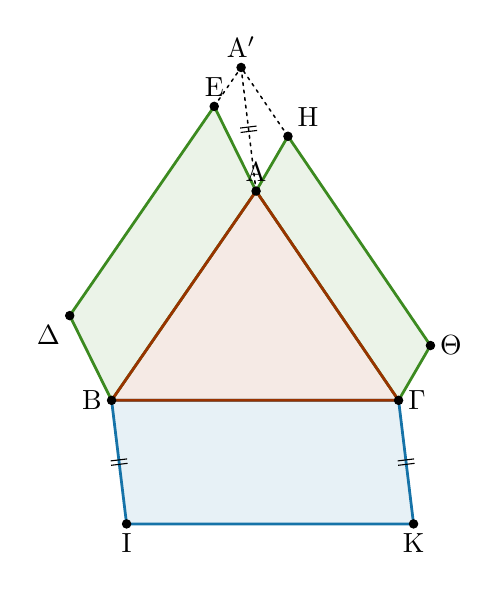
\begin{tikzpicture}[scale=.75]
\tkzSetUpLine[line width=1pt,color=black]
\tkzSetUpPoint[fill=black]

\def\Scale{1.35}
\FPeval{\Ax}{1.25 * \Scale}
\FPeval{\Ay}{3.6 * \Scale}
\FPeval{\Cx}{2.1 * \Ax}
\FPeval{\Ccx}{0.2 * \Scale}
\FPeval{\Cy}{1.45 * \Ax}
\FPeval{\Dx}{0.85 * \Ax}
\FPeval{\Dy}{(-1) * 0.42 * \Ax}
\FPeval{\Ty}{4 * \Scale}
\FPeval{\Tx}{0.55 * \Ax}

\tkzDefPoints{\Dy/\Dx/D,\Ay/0/C,\Cy/\Cx/B,0/0/A,\Ty/\Tx/Th}

\tkzDefParallelogram(B,A,D) \tkzGetPoint{E}
\tkzDefParallelogram(B,C,Th) \tkzGetPoint{H}

\tkzInterLL(D,E)(H,Th) \tkzGetPoint{A'}
\tkzDefPointWith[colinear= at A](A',B) \tkzGetPoint{I}
\tkzDefParallelogram(C,A,I) \tkzGetPoint{K}

\tkzFillPolygon[fill=ShapeClr,fill opacity=0.1](A,B,C)
\tkzFillPolygon[fill=GreenShapeClr,fill opacity=0.1](A,B,E,D)
\tkzFillPolygon[fill=GreenShapeClr,fill opacity=0.1](C,B,H,Th)
\tkzFillPolygon[fill=BlueShapeClr,fill opacity=0.1](A,C,K,I)

\tkzDrawSegment[line width=0.55pt,color=black](A,D)

\tkzDrawPolygon[color=GreenShapeClr](A,B,E,D)
\tkzDrawPolygon[color=GreenShapeClr](C,B,H,Th)
\tkzDrawPolygon[color=BlueShapeClr](A,C,K,I)
\tkzDrawPolygon[color=ShapeClr](A,B,C)

\tkzDrawSegments[line width=0.55pt,color=black,dashed,dash pattern=on 1pt off 1.75pt](E,A' H,A' A',B)

\tkzDrawPoints[size=3](A,B,C,D,E,H,Th,A',I,K)
\tkzLabelPoint[left](A){$\rm B$}
\tkzLabelPoint[above](B){$\rm A$}
\tkzLabelPoint[right](C){$\rm \Gamma$}
\tkzLabelPoint[below left](D){$\rm \Delta$}
\tkzLabelPoint[above](E){$\rm E$}
\tkzLabelPoint[right](Th){$\rm \Theta$}
\tkzLabelPoint[above right](H){$\rm H$}
\tkzLabelPoint[above](A'){$\rm A'$}
\tkzLabelPoint[below](I){$\rm I$}
\tkzLabelPoint[below](K){$\rm K$}

\tkzMarkSegments[mark=||,size=3](A',B A,I K,C)

\end{tikzpicture}
\end{document}
